\subsection{Git Workflow}
Git Workflow - это методология организации работы с репозиторием исходного кода.
Особенностью методологии является необходимость создавать отдельную ветку под
каждую задачу (issue-82, issue-85). Так же в репозитории присутствует хотя бы
одна центральная ветка (master) в которую сливаются изменения из ругих веток. В
крупных проектах могут присутствовать дополнительные центральные ветки,
предназначенные для объединения изменений перед тестированием продукта или
объединения изменений в процессе разработки. Введение дополнительных веток
позволяет работать на рабочей версией кода не обращая внимания на текущее
состояние разработки.

\begin{figure}[h]
\center{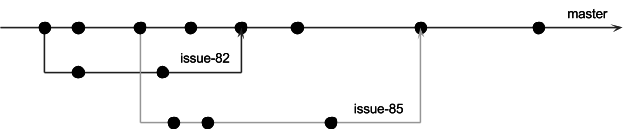
\includegraphics[width=1\linewidth]{one_central_branch.eps}}
\caption{Схема с одной центральной веткой.}
\label{ris:one_central_branch}
\end{figure}

В проекте использовались дополнительные центральные ветки для организации работы
над отдельной фазой. Со временем стало понятно что вести разработку в таком виде
сложно из-за того что необходимо было синхронизировать изменения в нескольких
центральных ветках. Так как проект еще не имел релизной версии, было принято
решение использовать одну центральную ветку (master) для всех задач (рис.
\ref{ris:one_central_branch}).
